\documentclass[a4paper,twoside]{article}

\usepackage{epsfig}
\usepackage{subfigure}
\usepackage{calc}
\usepackage{amssymb}
\usepackage{amstext}
\usepackage{amsmath}
\usepackage{amsthm}
\usepackage{multicol}
\usepackage{pslatex}
\usepackage{apalike}
\usepackage{SciTePress}
\usepackage[small]{caption}
\usepackage{epstopdf}
\usepackage[utf8]{inputenc}
\usepackage[ngerman,english]{babel}
\usepackage{graphicx}

\subfigtopskip=0pt
\subfigcapskip=0pt
\subfigbottomskip=0pt

\begin{document}

\title{\uppercase{Modellgetriebene Entwicklung einer mobilen Applikation mit JUSE4Android}}

\author{\authorname{Jano Espenhahn, Tobias Franz and Franziska Krebs}
\affiliation{Fachhochschule Brandenburg, Fachbereich Informatik und Medien}
\email{\{espenhah, franzt, krebsf\}@fh-brandenburg.de}
}

\keywords{MDA, UML, USE, OCL, Android}

\abstract{ein deutsches Abstract}{ein englisches Abstract}


\onecolumn \maketitle \normalsize \vfill

\section{\uppercase{Einleitung}}
\label{sec:introduction}

\subsection{Motivation}
\noindent Zitat Test
\cite{SilvaMasterThesis}
\subsection{Ziel}
\noindent 

\subsection{Aufgabenstellung}
\noindent 

\subsection{Abgrenzung}

\subsection{Ergebnis}

\section{\uppercase{JUSE4Android}}

\section{\uppercase{Vorstellung USE}}

UML based Specifiation Environment (USE) wird zur Spezifikation von Informationssystemen verwendet. Es basiert auf einer Teilmenge der Unified Modeling Language (UML). Eine USE-Spezifikation besteht aus einer textuellen Beschreibung eines Modells, bei der Eigenschaften aus UML-Diagramm verwendet werden. Um eine Spezifikation auf nicht-formale Anforderungen zu validieren, kann ein Modell mithilfe des USE-Tools animiert werden. Weitere Integritätsausdrücke für ein Modell können durch die Object Constraint Language (OCL) definiert werden. Die OCL wird im späteren Kapitel (TODO) vorgestellt. Die nachfolgende Abbildung veranschaulicht den Workflow für eine USE-Spezifikation.

\begin{figure}
	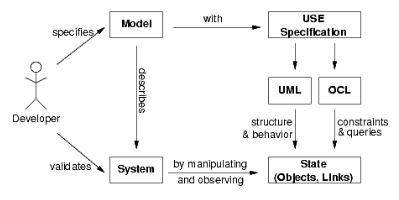
\includegraphics[scale=.7]{pics/USE_workflow.jpg}
	\caption{Workflow einer USE-Spezifikation}
\end{figure}

\subsection{Syntax}

\subsection{Tool}

\vfill
\bibliographystyle{apalike}
{\small
\bibliography{bib/literature}}

\section*{\uppercase{Anhang}}

\noindent If any, the appendix should appear directly after the
references without numbering, and not on a new page. To do so please use the following command:
\textit{$\backslash$section*\{APPENDIX\}}


\vfill
\end{document}

